\chapter{Метод анализа эпигенетических данных для оценки гендерных различий процесса старения человека}\label{ch:ch2}

\section{Входные данные}\label{sec:ch2/sec1}

Для анализа эпигенетических данных используется информация об уровнях метилирования CpG сайтов различных тканей человеческого организма. Среди множества существующих технологий сбора экспериментальных данных на данный момент наиболее распространённой технологией является массив Illumina Infinium HumanMethylation450 (450K) BeadChip, который покрывает более 480000 сайтов CpG и 96\% островов CpG в геноме человека \autocite{Bibikova2011}. Данная технология широко использовалась во многих крупных исследованиях, таких как The Cancer Genome Atlas (TCGA) и The International Cancer Genome Consortium (ICGC) Project \autocite{ICGC2010}. Благодаря доступности открытых банков данных, например, Gene Expression Omnibus (GEO) \autocite{Barrett2012}, за последние несколько лет стал доступным ряд методов анализа данных массива Illumina 450K.

В отличие от предыдущей платформы Illumina Infinium HumanMethylation27 (27K) BeadChip, в которой используется только один тип проб, Illumina 450K BeadChip включает два различных типа проб: Infinium I (n = 135501) и Infinium II (n = 350076) \autocite{Bibikova2011}, показанных на Рисунке~\ref{fig:infinium}. Каждый сайт CpG Infinium I характеризуется двумя пробами: одна для определения <<метилированной>> интенсивности (M --- methylated) и одна для определения <<неметилированной>> интенсивности (U --- unmethylated), тогда как каждый сайт CpG Infinium II использует только одну пробу, чтобы различать интенсивности <<M>> и <<U>> с помощью разные цветов (зелёный и красный). В таком случае значение $\beta$, характеризующее уровень метилирования одного сайта CpG, может быть вычислено как $\beta = M / (M + U + \alpha)$, где $\alpha = 100$. Также используется $M$-значение, $M = \log_2 (\beta / (1-\beta))$. Анализ данных, полученных с чипа Illumina, показывает, что Infinium II демонстрирует сдвиг значения в сторону увеличения для $\beta$ и в сторону уменьшения для $M$ \autocite{Dedeurwaerder2011}. Следовательно, предварительная обработка и нормализация имеют решающее значение для анализа данных массива Illumina 450K. 

\begin{figure}[ht]
	\centerfloat{
		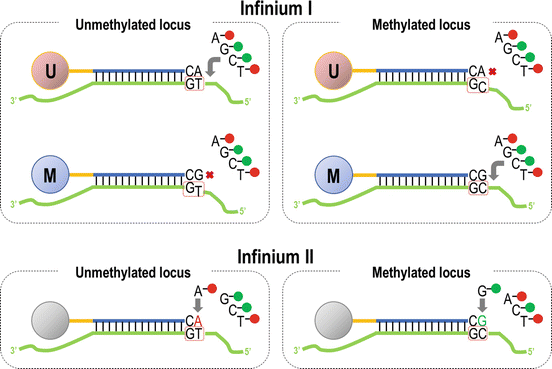
\includegraphics[scale=1.0]{infinium.png}
	}
	\caption[Пробы Infinium I и Infinium II.]{Пробы Infinium I и Infinium II \autocite{Nakabayashi2017}.}\label{fig:infinium}
\end{figure}

Процесс обработки данных метилирования, полученных с платформы Illumina (Рисунок~\ref{fig:pipeline}), включает обычно следующие шаги \autocite{Wang2018}: 
\begin{itemize}
	\item Импорт данных.
	\item Контроль качества.
	\item Нормализация внутри массива.
	\item Коррекция смещения.
	\item Идентификация различно метилированных проб и регионов.
	\item Биологическая интерпретация.
\end{itemize}

Существует две формы представления данных массива Illumina 450K: необработанные данные (*.idat), которые являются прямым выходом системы Illumina iScan и хранят интенсивности для каждого датчика; обработанные данные (*.txt), которые получаются после предварительной обработки. 

\begin{figure}[ht]
	\centerfloat{
		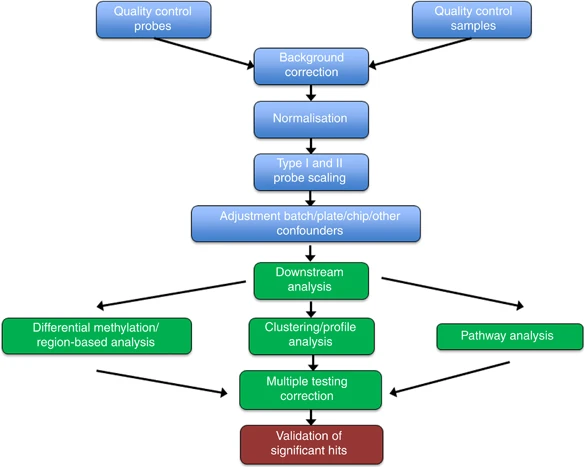
\includegraphics[scale=1.0]{pipeline.png}
	}
	\caption[Этапы обработки данных метилирования.]{Этапы обработки данных метилирования \autocite{WilhelmBenartzi2013}.}\label{fig:pipeline}
\end{figure}

После импорта данных следует оценить их качество. Во-первых, отфильтровываются пробы с высоким p-значением (например, $>0.05$). Во-вторых, в матрицу 450K встроено 850 контрольных проб, которые можно использовать для оценки интенсивности других проб. Образцы, не прошедшие этот контроль качества, исключаются из дальнейшего анализа. В-третьих, следует исключить из рассмотрения пробы на хромосомах X или Y, чтобы нивелировать влияние пола на анализ метилирования. В-четвёртых, $4.3~\%$ проб Illumina 450K содержат однонуклеотидный полиморфизм (SNP) на целевом сайте. Такие пробы могут вызывать проблемы при анализе взаимодействия проб \autocite{Price2013}. Также отфильтровываются перекрёстно-реактивные пробы на массиве Illumina 450K, поскольку значение $\beta$ на них с большей вероятностью представляет комбинацию нескольких сайтов \autocite{Zhou2016}.

Шаг нормализации включает коррекцию подложки и смещения цвета. Методы коррекции подложки основаны на моделях свёртки и используют out-of-band (OOB) интенсивности пробы \autocite{Triche2013}. Существует два основных метода, один из которых основан на датчиках отрицательного контроля, встроенных в BeadChip, а второй оценивает фон по режимам плотности интенсивности датчиков \autocite{Dedeurwaerder2011}. 

Смещение наиболее важно для исправления, поскольку оно является основным источником снижения качества данных. Поскольку пробы Infinium I более стабильны, большинство методов уменьшают смещение проб Infinium II, а не Infinium I. Один из наиболее распространённых методов называется коррекцией на основе пиков (PBC), который корректирует масштаб значений уровней метилирования Infinium II в границы распределения значений Infinium I. Однако, этот метод чувствителен к форме PDF значений $\beta$ и поэтому менее устойчив, когда распределение плотности не имеет чётко определённых пиков. Метод квантильной нормализации подмножества (SQN) основывается на предположении, что $\beta$-значения CpG, образующих одну и ту же биологическую категорию, должны иметь одинаковое распределение плотности \autocite{Touleimat2012}. Нормализация SWAN (Subset-quantile Within Array Normalization) \autocite{Maksimovic2012} была разработана на основе предположения, что распределение $\beta$-значений должно быть одинаковым, когда пробы имеют одинаковое количество CpG. Также важно устранить небиологические вариации, называемые групповые эффекты (batch effects), существующие между группами и отдельными образцами. Такие эффекты могут влиять на измерения и могут быть частично устранены путём нормализации между выборками с использованием анализа главных компонент.

Информация обо всех измеряемых пробах CpG содержится в файле аннотаций Infinium --- имя CpG, хромосома, регион, принадлежность гену и острову CpG. Касательно расположения относительно острова CpG, пробы классифицируются на четыре категории: сайты, расположенные внутри острова; пробы, расположенные на берегах острова (0-2000 bp); пробы, расположенные на шельфах (2000-4000 bp) и пробы, расположенные в <<открытом море>>. Касательно их отношения к аннотированным генам, пробы классифицируются как внутри промотора, внутри области 5'-UTR, внутри тела гена и внутри области 3'-UTR. 

Таким образом, сырые данные метилирования были обработаны в соответствии с вышеобозначенными шагами: уровни метилирования были нормализованы, необходимые пробы отфильтрованы. Если данные были уже нормализованы авторами соответствующих работ, то проводилось только фильтрование некорректных проб. В результате работа проводилась с тремя основными типами данных: таблица с уровнями метилирования, аннотации и атрибуты субъектов. Уровни метилирования представляют собой таблицу с $\beta$-значениями, по столбцам которой отмечены субъекты, по строкам --- сайты CpG. Также доступна информация о субъектах --- возраст, пол, дополнительные характеристики (вес, рост, вредные привычки). Информация обо всех сайтах CpG одинакова для всех проводимых экспериментов, и предоставляется производителем чипов Illumina.

Для проверки результатов работы предлагаемых алгоритмов использовались 4 набора данных метилирования цельной крови человека, полученных с помощью платформы Illumina 450K. Поиск данных, находящихся в открытом доступе, производился с помощью репозитория наборов данных Gene Expression Omnibus (GEO) \autocite{Barrett2012}. Были выбраны наборы данных метилирования цельной крови, содержащие информацию о поле и возрасте, с наибольшим количеством здоровых субъектов: GSE40279 \autocite{Hannum2013}, GSE87571 \autocite{Johansson2013} и GSE55763 \autocite{Lehne2015}. Кроме того, был рассмотрен четвёртый набор данных, не загруженный в GEO, являющийся частью исследования EPIC Italy \autocite{Palli2003}. Общее количество рассматриваемых субъектов в каждом наборе данных, количество мужчин и женщин, а также возрастной диапазон, представлены в Таблице~\ref{tab:Datasets}. 

\begin{table} [htbp]
	\centering
	\begin{threeparttable}
		\caption{Характеристики рассматриваемых наборов данных Illumina 450k}\label{tab:Datasets}
		\begin{SingleSpace}
			\begin{tabular}{| l | c | c | c | c |}
				\hline
				 & GSE40279 & GSE87571 & EPIC & GSE55763 \\
				\hline
				Количество субъектов & 656 & 729 & 1803 & 2670 \\
				\hline
				Количество женщин & 338 & 388 & 1114 & 860 \\
				\hline
				Количество мужчин & 318 & 341 & 689 & 1810 \\
				\hline
				Возрастной диапазон & 19-101 & 14-94 & 34-74 & 35-75 \\
				\hline
			\end{tabular}%
		\end{SingleSpace}
	\end{threeparttable}
\end{table}

Пробы на половых хромосомах, пробы с внутренними SNP и с неуникальным картированием в бисульфит-преобразованном геноме согласно \autocite{Zhou2016} были исключены из рассмотрения. В результате осталось 414505 проб для GSE40279, 414950 проб для GSE87571, 349534 пробы для EPIC и 382458 проб для GSE55763. 

\section{Метод поиска связанных с возрастом специфичных для пола биомаркеров}\label{sec:ch2/sec2}

\subsection{Описание алгоритма}\label{subsec:ch2/sec2/subsec1}

Опишем алгоритм для определения биомаркеров, имеющих зависимость как от категориальных, так и от непрерывных переменных. Предполагается, что в качестве входа используются несколько баз данных метилирования, полученных из различных источников (собранных в различных лабораторных условиях в рамках разных исследований) и представленных в виде таблиц, описанных в разделе \ref{sec:ch2/sec1} --- таблицы значений уровней метилирования, информации о субъектах и информации о сайтах CpG. Эти данные могут быть взяты из одинаковых, либо из различных органов и тканей организма человека. 

Для данных метилирования цельной крови первоначально проводится коррекция с учётом клеточного состава. Пропорции клеток цельной крови (клетки CD4T, CD8T, NK, B-клетки и гранулоциты) были получены с использованием метода, описанного в работе \autocite{Horvath2013}. Для того, чтобы исключить влияние клеточного состава на уровень метилирования, для каждого сайта CpG применяется модель линейной регрессии, согласно формуле:
\begin{equation}
\label{eq:cell_correction}
\beta \sim \text{CD4T} + \text{CD8T} + \text{NK} + \text{B-cell} + \text{Gran},
\end{equation}
где в левой части $\beta$ --- уровень метилирования, в правой части --- пропорции соответствующих клеток крови. Скорректированные уровни метилирования представляют собой невязки построенной линейной регрессии.

Задачей, решаемой с помощью предлагаемого алгоритма, является поиск сайтов CpG, демонстрирующих одновременно и различия в метилировании ДНК между двумя полами, и возрастные изменения в уровне метилирования ДНК (поиск связанных с полом и возрастом различно метилированных позиций, sex-specific age-related differentially methylated probes, далее обозначаемых как saDMP). 

Алгоритм предполагает выполнение следующих шагов \autocite{Yusipov2020}:
\begin{enumerate}
	\item Сначала для каждого набора данных проводится коррекция значений уровней метилирования с учётом возраста (если данные метилирования для цельной крови, то они должны быть скорректированы с учётом клеточного состава). Для этого к каждому сайту CpG у каждого субъекта применяется модель линейной регрессии, аналогичная формуле \ref{eq:cell_correction}, в правой части которой находится значение возраста. Далее, в каждом наборе данных для каждого сайта CpG вычисляется коэффициент корреляции Пирсона \autocite{royal1895proceedings} между полом и уровнем метилирования, а также соответствующее p-значение. Для полученного списка p-значений проводится поправка на множественную проверку гипотез согласно алгоритму Бенждамини-Хохберга \autocite{Benjamini1995}. Алгоритм METAL \autocite{Willer2010} используется для выполнения взвешенного по размеру выборки метаанализа для списков скорректированных p-значений всех рассматриваемых наборов данных одновременно в соответствии с формулами \ref{eq:metal_z} и \ref{eq:metal_p}. Таким образом, получается список проб с зависимыми от пола паттернами уровня метилирования (sex-specific differentially methylated probes, далее обозначаемые как sDMP).
	\item Далее для каждого набора данных проводится коррекция значений уровней метилирования с учётом пола (если данные метилирования для цельной крови, то они должны быть скорректированы с учётом клеточного состава). Для этого к каждому сайту CpG у каждого субъекта применяется модель линейной регрессии, аналогичная формуле \ref{eq:cell_correction}, в правой части которой находится пол (закодированный в числовом виде). Далее, в каждом наборе данных для каждого сайта CpG вычисляется коэффициент корреляции Пирсона \autocite{royal1895proceedings} между возрастом и уровнем метилирования, а также соответствующее p-значение. Для полученного списка p-значений проводится поправка на множественную проверку гипотез согласно алгоритму Бенждамини-Хохберга \autocite{Benjamini1995}. Алгоритм METAL \autocite{Willer2010} используется для выполнения взвешенного по размеру выборки метаанализа для списков скорректированных p-значений всех рассматриваемых наборов данных одновременно в соответствии с формулами \ref{eq:metal_z} и \ref{eq:metal_p}. Таким образом, получается список проб с зависимыми от возраста паттернами уровня метилирования (age-related differentially methylated probes, далее обозначаемые как aDMP).
	\item Для полученных с помощью метаанализа p-значений проводится поправка на множественную проверку гипотез согласно алгоритму Бонферрони \autocite{bonferroni1936teoria}. Отбираются только пробы с согласованными паттернами во всех наборах данных (для sDMP: гиперметилированные или гипометилированные у мужчин по сравнению с женщинами во всех наборах данных; для aDMP: гиперметилированные или гипометилированные с возрастом во всех наборах данных).
	\item Получение пересечённого списка из списков проб с зависимыми от пола паттернами уровня метилирования (sDMP) и проб с зависимыми от возраста паттернами уровня метилирования (aDMP), в результате имеется список связанных с возрастом и специфичных для пола различно метилированных позиций (saDMP).
\end{enumerate}

Также для всех наборов данных можно рассмотреть статистику эпигенетических мутаций, или эпимутаций. Эпимутация определяется как аномальное подавление транскрипции активных генов (экспрессия которых обычно не подавляется) или аномальная активация репрессированных генов (экспрессия которых обычно подавляется), вызванная ошибками в эпигенетической репрессии генов. Эпимутация возникает в соматических клетках. С точки зрения метилирования ДНК, эпимутации представляют собой такие сайты CpG, для которых один или несколько субъектов демонстрируют аномально отличающиеся от остальной популяции уровни метилирования. Для того, чтобы обнаружить эпимутации, для каждого сайта CpG для всех субъектов строится распределение значений уровней метилирования, вычисляются первый и третий квартили Q1 и Q3, а также межквартильный интервал $\text{IQR} = \text{Q3} - \text{Q1}$ \autocite{Gentilini2015}. Если для данного сайта CpG значение уровня метилирования $\beta$ у одного или нескольких субъектов превышает межквартильный интервал в три раза:
\begin{equation}
\label{eq:iqr}
\text{Q1} - (3 \times \text{IQR}); \text{Q3} + (3 \times \text{IQR}), 
\end{equation}
то в нём наблюдается эпимутация у рассматриваемых субъектов. Увеличенный уровень накопления эпимутаций у отдельно взятого субъекта может свидетельствовать об ускоренном старении и различных заболеваниях.

\subsection{Результаты работы метода на реальных данных}\label{subsec:ch2/sec2/subsec2}

К четырём рассматриваемым большим наборам данных метилирования цельной крови (Таблица~\ref{tab:Datasets}) был применён алгоритм, описанный в разделе \ref{subsec:ch2/sec2/subsec1}. Сначала были выявлены сайты CpG с различными паттернами метилирования у мужчин и женщин (sDMP) --- 38100 проб было получено в результате метаанализа со скорректированными в соответствии с процедурой Бонферрони p-значениями $< 0.01$. Среди полученных проб $53~\%$ были гиперметилированы у женщин по сравнению с мужчинами. Затем были выявлены сайты CpG с возрастными тенденциями изменения уровня метилирования (aDMP) --- 87571 проба была получена в результате метаанализа со скорректированными в соответствии с процедурой Бонферрони p-значениями $< 0.01$. Среди полученных проб $52~\%$ были гиперметилированы с возрастом. Далее мы проверили, сколько sDMP имеют возрастные тенденции изменения уровня метилирования, т.е. также являются aDMP. Пересечение списков sDMP и aDMP дало 16526 проб, связанных одновременно с полом и возрастом. Было также обнаружено, что большинство saDMP, имеющие тенденции к гипометилированию с возрастом, являются более метилированными у мужчин по сравнению с женщинами, в то время как большинство гиперметилированных с возрастом saDMP являются более метилированными у женщин по сравнению с мужчинами (Рисунок~\ref{fig:saDMP}).

\begin{figure}[ht]
	\centerfloat{
		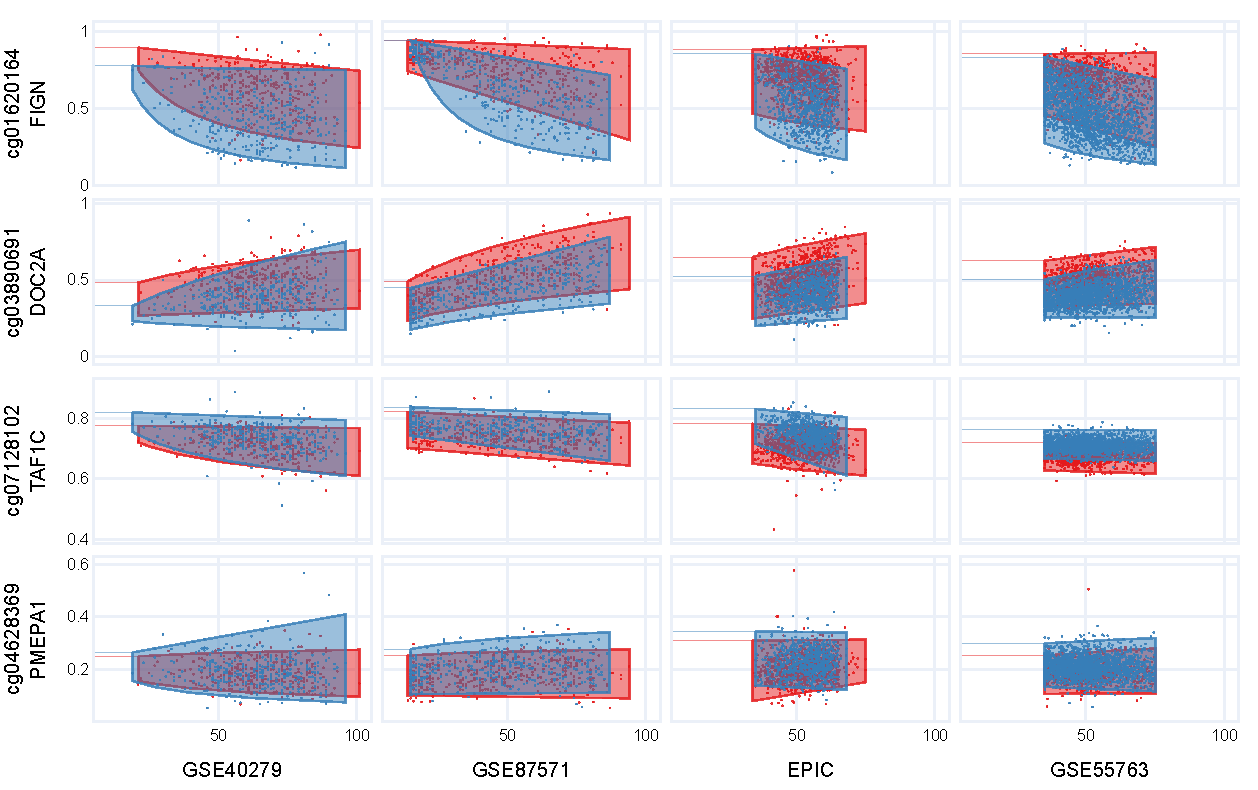
\includegraphics[scale=0.8]{saDMP.pdf}
	}
	\caption[Диаграммы разброса отдельных saDMP в четырёх рассматриваемых наборах данных.]{Диаграммы разброса отдельных saDMP в четырёх рассматриваемых наборах данных: cg01620164 гипометилирован у мужчин и гипометилирован с возрастом; cg03890691 гипометилирован у мужчин и гиперметилирован с возрастом; cg07128102 гиперметилирован у мужчин и гипометилирован с возрастом; cg04628369 гиперметилирован у мужчин и гиперметилирован с возрастом. Красные точки обозначают субъектов женского пола, синие --- мужского \autocite{Yusipov2020}.}\label{fig:saDMP}
\end{figure}

Этот результат предполагает, что сайты CpG, демонстрирующие различия между мужчинами и женщинами, особенно склонны к эпигенетическим изменениям во время старения. Полученный список saDMP был обогащён множеством генных функций, связанных с нейрональными функциями и межклеточными взаимодействиями. Однако, пробы, связанные с полом, но не возрастом, не были обогащены каким-либо конкретным биологическим процессом. При сравнении с ранее опубликованными результатами было обнаружено, что 1121 saDMP были обнаружены ранее как имеющие половые различия в уровне метилирования (вне зависимости от возраста) \autocite{Inoshita2015, Singmann2015, Yousefi2015}. Также был проведён точный тест Фишера \autocite{fisher2006statistical} на обогащение определённых хромосом, островов CpG и генных регионов найденными saDMP (Рисунок~\ref{fig:saDMP_Fisher}). Хромосомы 1, 5. 20 были значительно обогащены saDMP (с p-значением теста Фишера $< 0.05$), в то время как хромосомы 7, 8, 16, 21 были значительно истощены saDMP (с p-значением теста Фишера $< 0.02$). Также побережья островов CpG (и северные, и южные) были значительно обогащены saDMP (с p-значением теста Фишера $< 1 \cdot 10^{-32}$), в то время как шельфы были значительно истощены saDMP (с p-значением теста Фишера $< 1 \cdot 10^{-3}$). Регион TSS1500 и тело генов были значительно обогащены saDMP (с p-значением теста Фишера $< 1 \cdot 10^{-7}$), в то время как регионы TS200 и 1stExon были значительно истощены saDMP (с p-значением теста Фишера $< 1 \cdot 10^{-18}$). Список saDMP также включает высокую долю генов, связанных с гормонами, но обогащение не было статистически значимым.

\begin{figure}[ht]
	\begin{minipage}[b][][b]{0.49\linewidth}\centering
		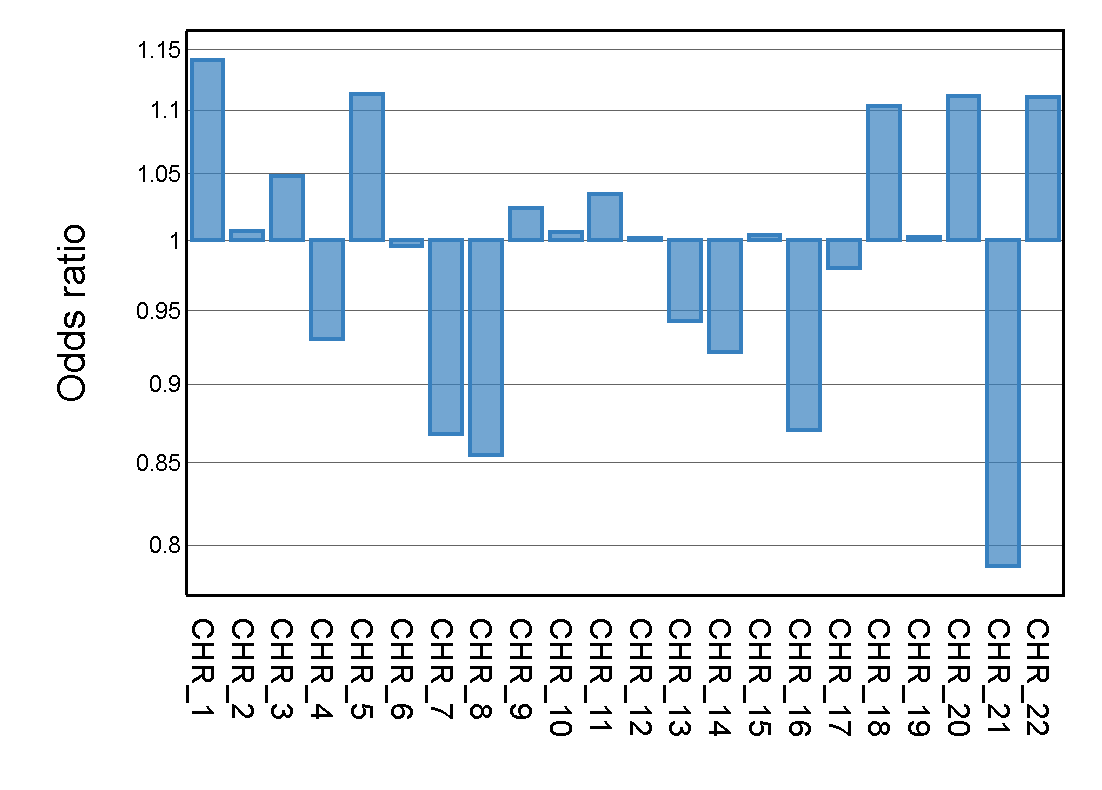
\includegraphics[width=0.99\linewidth]{saDMP_chr.pdf} \\ а)
	\end{minipage}
	\hfill
	\begin{minipage}[b][][b]{0.49\linewidth}\centering
		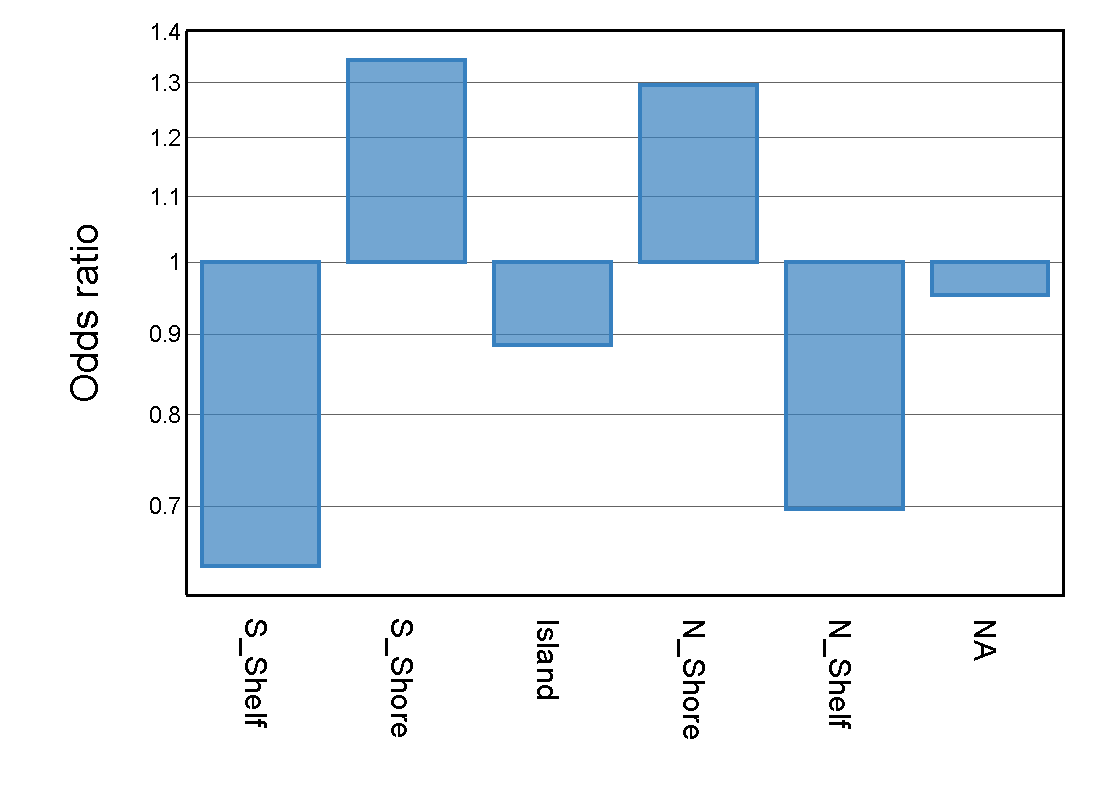
\includegraphics[width=0.99\linewidth]{saDMP_island.pdf} \\ б)
	\end{minipage}
	\begin{minipage}[b][][b]{0.99\linewidth}\centering
		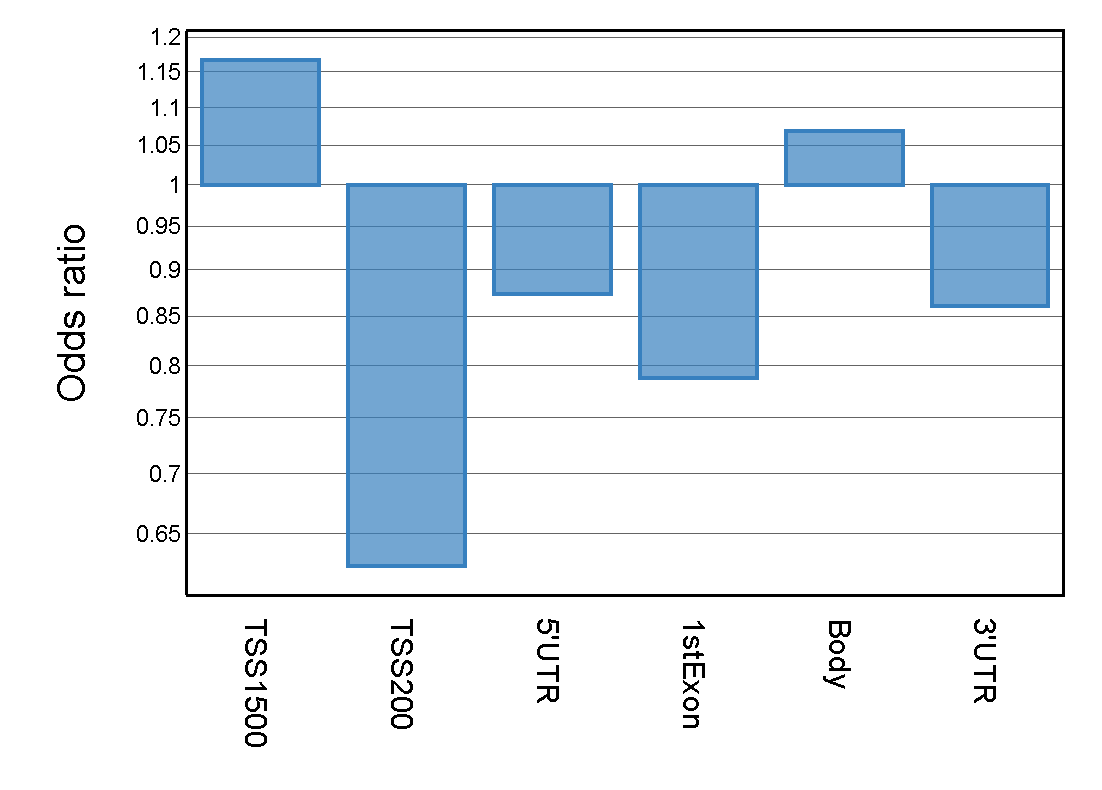
\includegraphics[width=0.485\linewidth]{saDMP_gene.pdf} \\ в)
	\end{minipage}
	\caption[Обогащение найденными saDMP хромосом, островов CpG и генных регионов.]{Обогащение (отношение шансов) найденными saDMP (а) хромосом, (б) островов CpG и (в) генных регионов.}
	\label{fig:saDMP_Fisher}
\end{figure}

Также были оценены связанные с полом и возрастом паттерны во всех 4 наборах данных. Метаанализ привёл к получению 8 сайтов CpG, метилирование которых показало разные траектории старения в зависимости от пола (Таблица~\ref{tab:saDMP}). Наиболее значимый сайт CpG (cg18834375) располагается в гене FIGN, который также занимал первое место в списке saDMP и включает множественные сайты CpG, демонстрирующие разные уровни метилирования в зависимости от пола и возраста (cg01620164, cg19156483, cg10864319, cg18834375, cg15259986 и cg03878133).

\begin{table} [htbp]
	\centering
	\begin{threeparttable}
		\caption{Сайты CpG, связанные с полом и возрастом в рассматриваемых наборах данных}\label{tab:saDMP}
		\begin{SingleSpace}
			\begin{tabular}{| l | c | c | c | }
				\hline
				CpG & Хромосома & Ген & p-значение метаанализа \\
				\hline
				cg18834375 & 2 & FIGN & $4.98 \cdot 10^{-08}$ \\
				\hline
				cg08726667 & 16 & CCDC101 & $2.54 \cdot 10^{-07}$ \\
				\hline
				cg25748357 & 7 & GRB10 & $4.78 \cdot 10^{-04}$  \\
				\hline
				cg19458410 & 21 & RCAN1 & $5.51 \cdot 10^{-04}$ \\
				\hline
				cg26227957 & 1 & KIAA0090 & $6.43 \cdot 10^{-04}$ \\
				\hline
				cg25291941 & 8 & POP1 & $4.22 \cdot 10^{-03}$ \\
				\hline
				cg12050508 & 6 & TNFAIP3 & $5.31 \cdot 10^{-03}$ \\
				\hline
				cg13091627 & 1 & S100A4 & $6.85 \cdot 10^{-03}$ \\
				\hline
			\end{tabular}%
		\end{SingleSpace}
	\end{threeparttable}
\end{table}

Вычисление количества эпимутаций для каждого набора данных показало, что оно увеличивается с возрастом как у мужчин так и у женщин, однако, половых тенденций не наблюдалось (Рисунок~\ref{fig:epimutations}). 

\begin{figure}[ht]
	\centerfloat{
		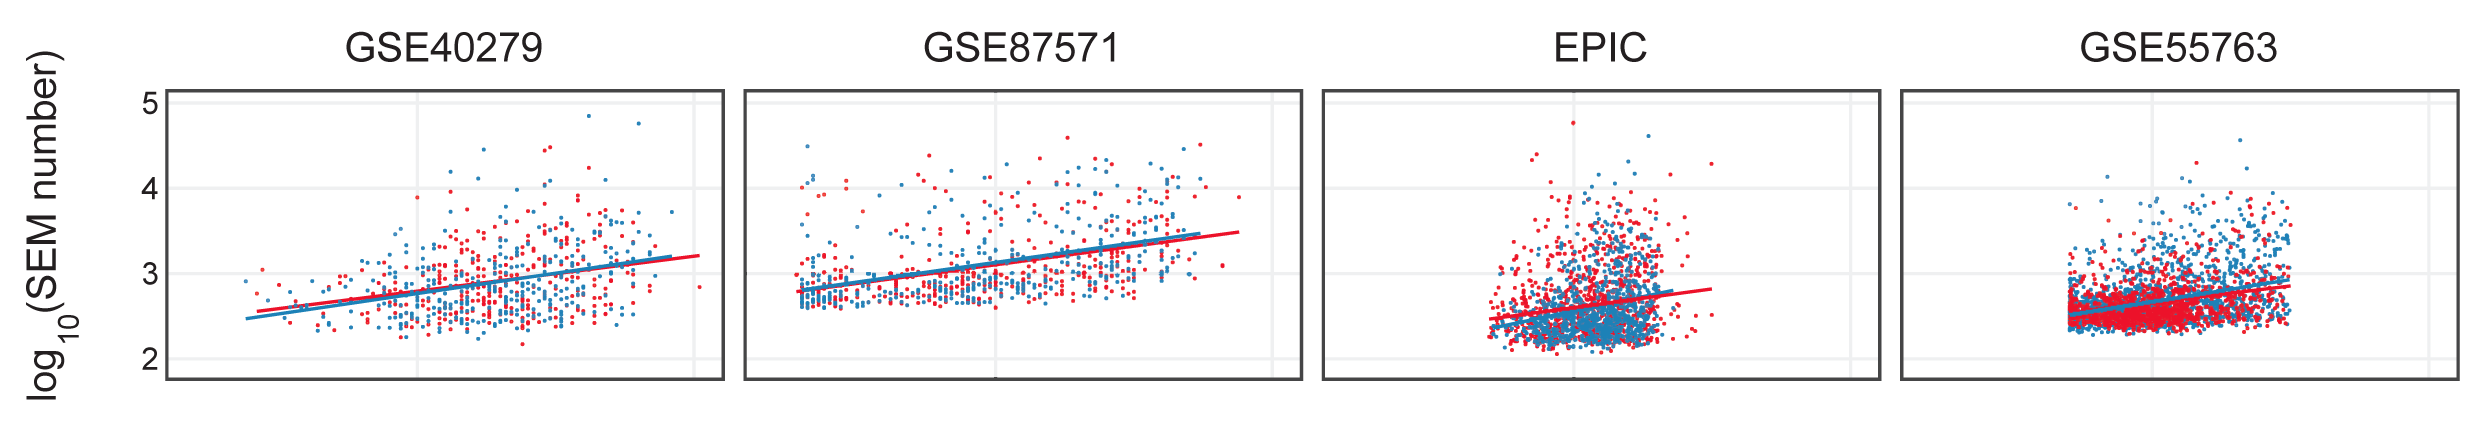
\includegraphics[scale=0.27]{epimutations.png}
	}
	\caption[Количество эпимутаций (в логарифмической шкале) в зависимости от возраста у женщин и мужчин.]{Количество эпимутаций (в логарифмической шкале) в зависимости от возраста у женщин (красный) и мужчин (синий) \autocite{Yusipov2020}.}\label{fig:epimutations}
\end{figure}

\section{Метод поиска биомаркеров с возрастной вариабельностью, связанной с полом}\label{sec:ch2/sec3}

\subsection{Описание алгоритма}\label{subsec:ch2/sec3/subsec1}

Опишем алгоритм для определения биомаркеров, имеющих изменение вариабельности, зависимой как от категориальных, так и от независимых переменных. Под вариабельностью уровней метилирования в данном случае понимается различие их значений у рассматриваемых субъектов за некоторый промежуток времени. В зависимости от возраста вариабельность предполагает изменение дисперсии для группы субъектов в разных возрастных диапазонах. Предполагается, что в качестве входа используются базы данных метилирования, представленные в виде таблиц, описанных в разделе \ref{sec:ch2/sec1}. Эти данные могут соответствовать одним и тем же, либо различным органам и тканям организма человека. 

Аналогично алгоритму для определения биомаркеров, связанных с возрастом и специфичных для пола, описанному ранее (см. Раздел~\ref{subsec:ch2/sec2/subsec1}), для данных цельной крови проводится коррекция значений уровней метилирования с учётом клеточного состава согласно формуле \ref{eq:cell_correction}. Скорректированные уровни метилирования представляют собой невязки построенной линейной регрессии.

Задачей, решаемой с помощью предлагаемого алгоритма, является поиск таких сайтов CpG, демонстрирующих одновременно и различия в вариабельности уровней метилирования ДНК между двумя полами, и возрастные изменения вариабельности уровня метилирования ДНК (поиск связанных с полом и возрастом различно вариабельных метилированных позиций, saVMP).

Алгоритм предполагает выполнение следующих шагов \autocite{Yusipov2020}:
\begin{enumerate}
	\item Сначала каждый набор данных (если данные метилирования цельной крови, то они должны быть скорректированы с учётом клеточного состава) разделяется на два подмножества --- женщины и мужчины отдельно. Для каждого из подмножеств проводится проверка уровней метилирования на гетероскедастичность относительно возраста (вектор является гетероскедастичным, если дисперсия ошибки изменяется для различных элементов вектора). Для этого используется тест Бройша-Пагана \autocite{Breusch1979, COOK1983}, также вычисляются соответствующие p-значения.
	\item К полученному списку p-значений применяется алгоритм METAL \autocite{Willer2010} для выполнения взвешенного по размеру выборки метаанализа отдельно для каждого подмножества --- женщин и мужчин. Для полученных с помощью метаанализа p-значений проводится поправка на множественную проверку гипотез согласно алгоритму Бонферрони \autocite{bonferroni1936teoria}. Отбираются те сайты CpG, скорректированное p-значение которых преодолевает порог значимости $0.01$.
	\item Существует 3 основных сценария половых различий в возрастной вариабельности уровней метилирования ДНК:
	\begin{itemize}
		\item Проба является гетероскедастичной у женщин и гомоскедастичной у мужчин, то есть проба с метаанализированным и скорректированным алгоритмом Бонферрони p-значением меньше $0.01$ у женщин и больше $0.05$ у мужчин.  
		\item Проба является гомоскедастичной у женщин и гетероскедастичной у мужчин, то есть проба с метаанализированным и скорректированным алгоритмом Бонферрони p-значением меньше $0.01$ у мужчин и больше $0.05$ у женщин.
		\item Проба является гетероскедастичной как у женщин, так и мужчин, но с противоположным направлением изменения вариабельности (вариабельность увеличивается у женщин и уменьшается у мужчин, либо вариабельность уменьшается у женщин и увеличивается у мужчин).
	\end{itemize}
\end{enumerate}

\subsection{Результаты работы метода на реальных данных}\label{subsec:ch2/sec3/subsec2}

К четырём рассматриваемым большим наборам данных метилирования цельной крови (Таблица~\ref{tab:Datasets}) был применён алгоритм, описанный в разделе \ref{subsec:ch2/sec3/subsec1}. Было выявлено 809 и 12178 проб CpG, имеющих специфичные паттерны вариабельности для женщин и мужчин соответственно (saVMP), примеры изображены на Рисунке~\ref{fig:saVMP}. Все специфичные для женщин saVMP показали увеличение вариабельности с возрастом, только 5 из 12178 специфичных для мужчин saVMP имеют уменьшение вариабельности уровня метилирования с возрастом. Не было выявлено ни одной пробы CpG с противоположными тенденциями изменения вариабельности уровня метилирования у обоих полов. 

\begin{figure}[ht]
	\begin{minipage}[b][][b]{0.49\linewidth}\centering
		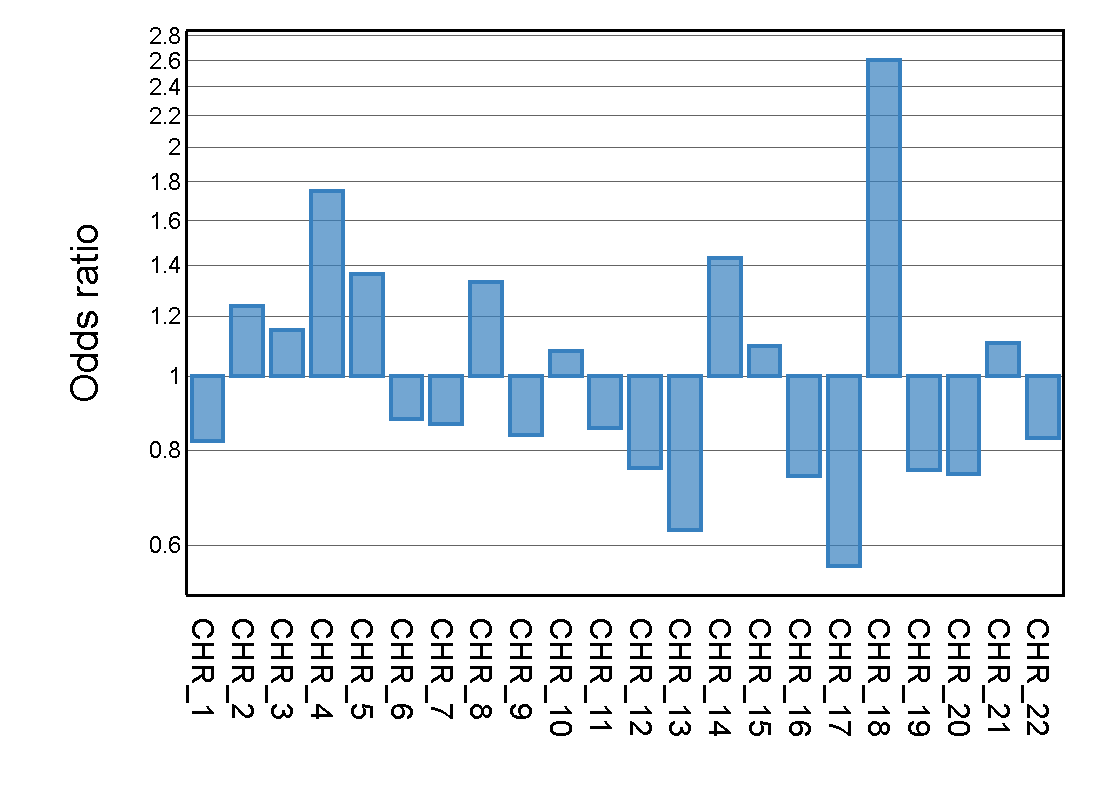
\includegraphics[width=0.99\linewidth]{saVMP_chr_f.pdf} \\ а)
	\end{minipage}
	\hfill
	\begin{minipage}[b][][b]{0.49\linewidth}\centering
		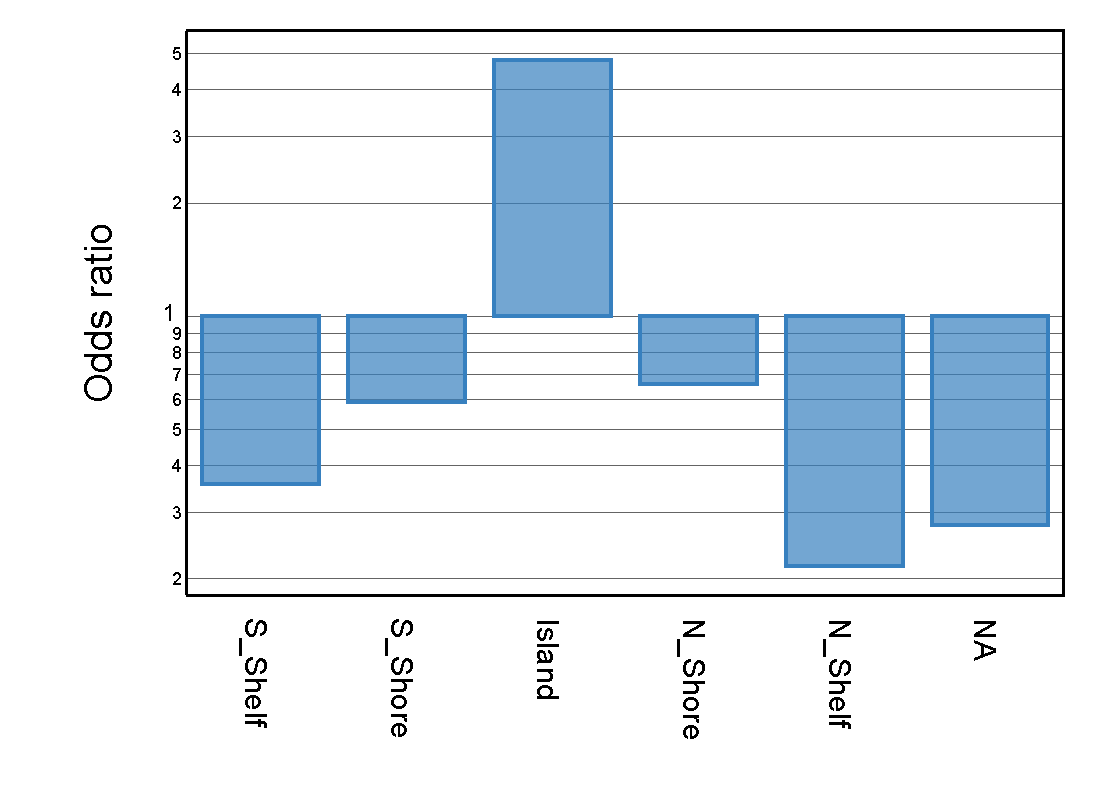
\includegraphics[width=0.99\linewidth]{saVMP_island_f.pdf} \\ б)
	\end{minipage}
	\begin{minipage}[b][][b]{0.99\linewidth}\centering
		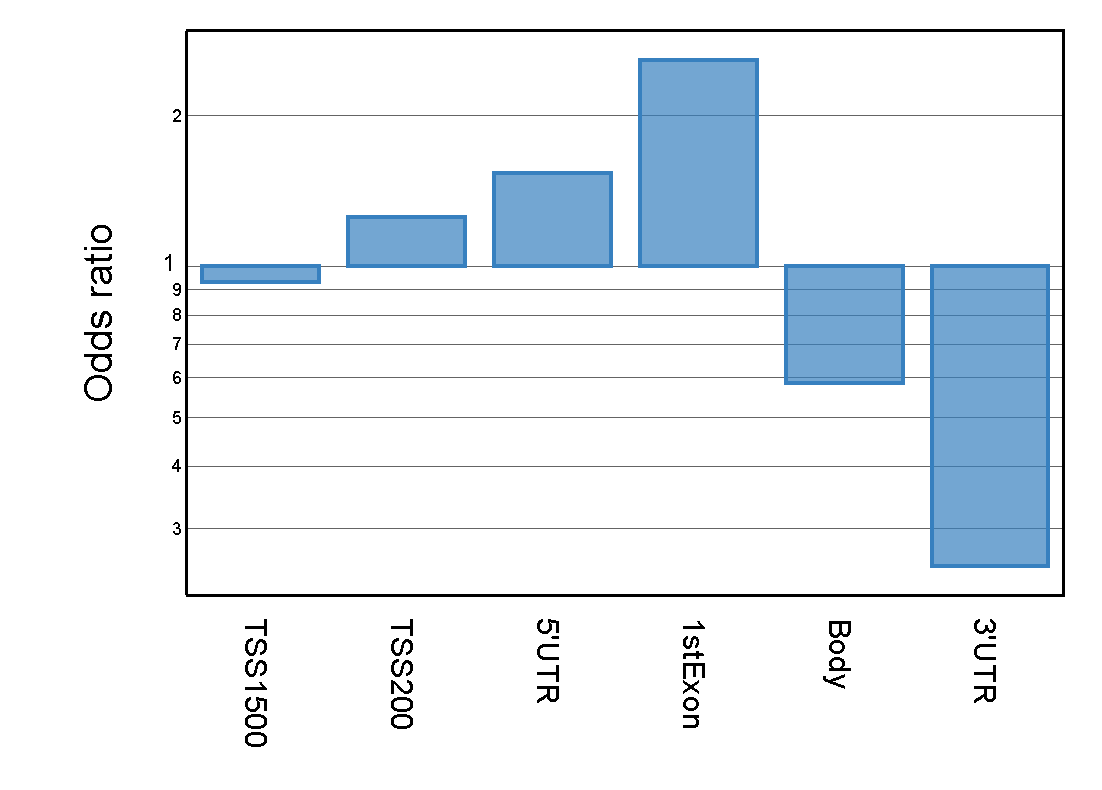
\includegraphics[width=0.485\linewidth]{saVMP_gene_f.pdf} \\ в)
	\end{minipage}
	\caption[Обогащение найденными saVMP, специфичными для женщин, хромосом, островов CpG и генных регионов.]{Обогащение (отношение шансов) найденными saVMP, специфичными для женщин, (а) хромосом, (б) островов CpG и (в) генных регионов.}
	\label{fig:saVMP_Fisher_f}
\end{figure}

Также был проведён точный тест Фишера \autocite{fisher2006statistical} на обогащение определённых хромосом, островов CpG и генных регионов найденными saVMP, специфичных для женщин (Рисунок~\ref{fig:saVMP_Fisher_f}) и для мужчин (Рисунок~\ref{fig:saVMP_Fisher_m}). Хромосомы 4, 5, 14, 18 были значительно обогащены saVMP (с p-значением теста Фишера $< 0.05$) у женщин, а хромосомы 5, 14, 16, 18, 19, 20 (с p-значением теста Фишера $< 0.02$) --- у мужчин. Хромосомы 14 и 18 обогащены saVMP как у женщин, так и у мужчин. В то же время хромосома 17 была значительно истощена saVMP (с p-значением теста Фишера $< 0.001$) у женщин, а хромосомы 1, 3, 6, 7, 22, 17, 21, 22 (с p-значением теста Фишера $< 0.05$) -- у мужчин. Острова CpG были значительно обогащены saVMP (с p-значением теста Фишера $< 1 \cdot 10^{-5}$) у женщин, а северные и южные побережья (с p-значением теста Фишера $< 1 \cdot 10^{-88}$) --- у мужчин. В то же время побережья островов CpG и шельфы были значительно истощены saVMP (с p-значением теста Фишера $< 0.001$) у женщин, а острова CpG и шельфы (с p-значением теста Фишера $< 1 \cdot 10^{-10}$) -- у мужчин. Шельфы островов CpG истощены saVMP как у женщин, так и у мужчин. Такие генные регионы как TSS200, 5'UTR и 1stExon были значительно обогащены saVMP (с p-значением теста Фишера $< 0.005$) у женщин, а TSS1500 (с p-значением теста Фишера $< 1 \cdot 10^{-10}$) --- у мужчин. В то же время тела генов и 3'UTR были значительно истощены saVMP (с p-значением теста Фишера $< 1 \cdot 10^{-10}$) у женщин, а TSS200, 5'UTR, 1stExon, 3'UTR и тела генов (с p-значением теста Фишера $< 1 \cdot 10^{-8}$) -- у мужчин. Тела генов и 3'UTR истощены saVMP как у женщин, так и у мужчин.

\begin{figure}[ht]
	\begin{minipage}[b][][b]{0.49\linewidth}\centering
		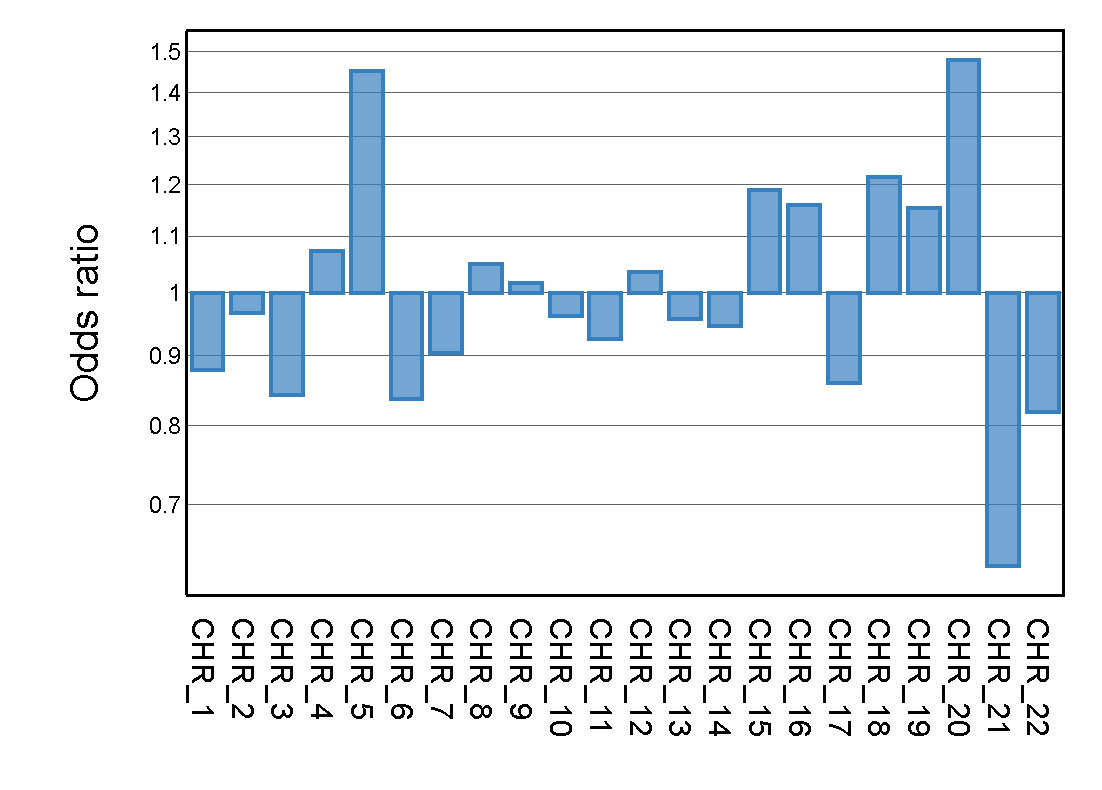
\includegraphics[width=0.99\linewidth]{saVMP_chr_m.pdf} \\ а)
	\end{minipage}
	\hfill
	\begin{minipage}[b][][b]{0.49\linewidth}\centering
		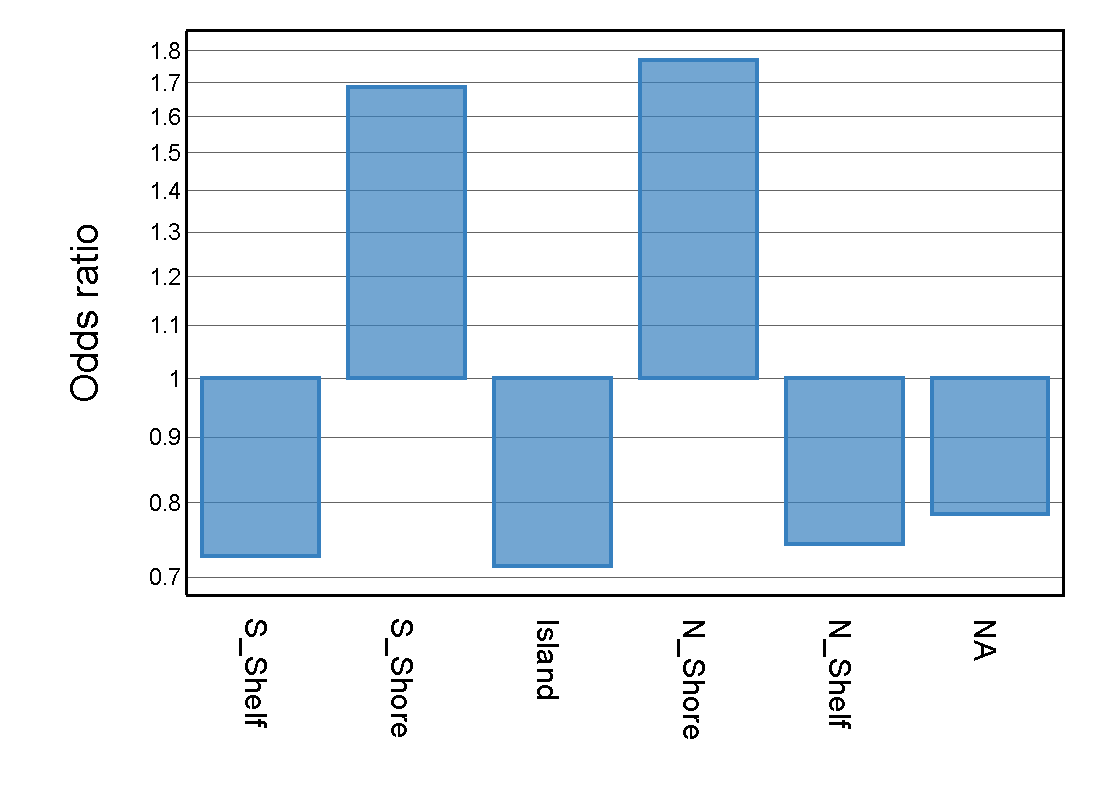
\includegraphics[width=0.99\linewidth]{saVMP_island_m.pdf} \\ б)
	\end{minipage}
	\begin{minipage}[b][][b]{0.99\linewidth}\centering
		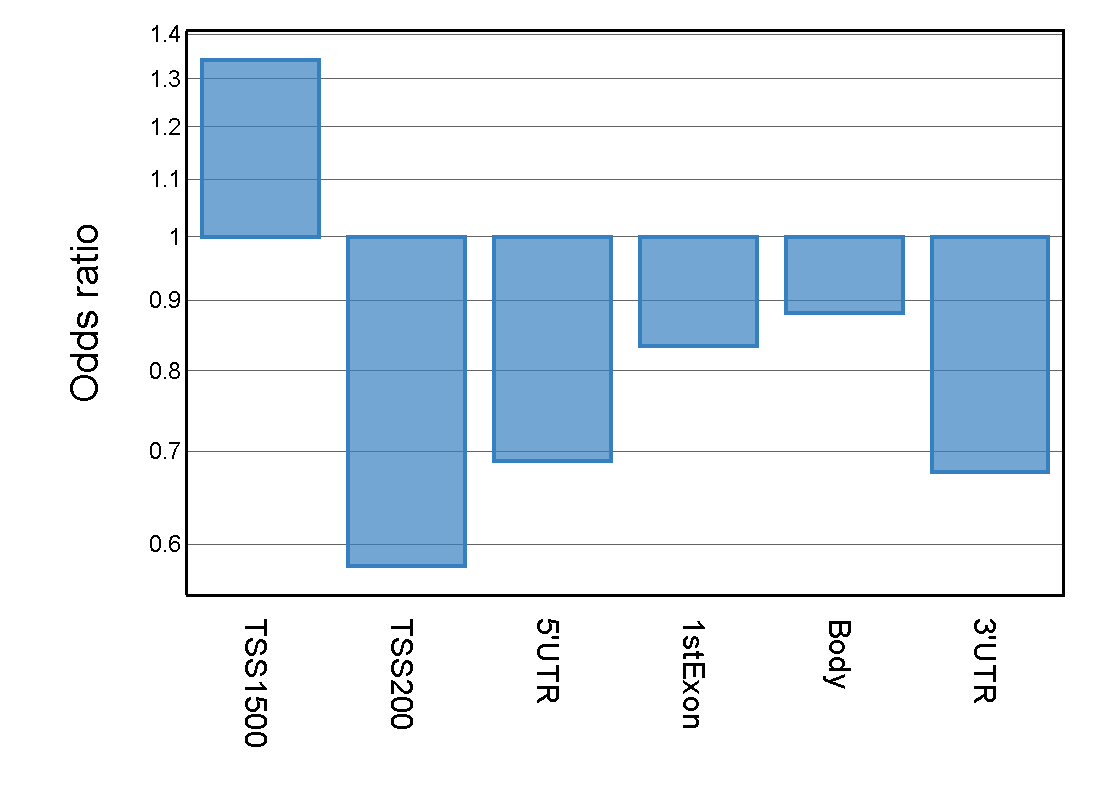
\includegraphics[width=0.485\linewidth]{saVMP_gene_m.pdf} \\ в)
	\end{minipage}
	\caption[Обогащение найденными saVMP, специфичными для мужчин, хромосом, островов CpG и генных регионов.]{Обогащение (отношение шансов) найденными saVMP, специфичными для мужчин, (а) хромосом, (б) островов CpG и (в) генных регионов.}
	\label{fig:saVMP_Fisher_m}
\end{figure}

Как женские, так и мужские saVMP были обогащены несколькими функциями генов, связанных с нейрональными процессами и процессами развития. Также оказалось, что специфические для мужчин saVMP обогащали гены, связанных с выработкой гормонов, хотя это обогащение не было значимым. Увеличение эпигенетической вариабельности в процессе старения наблюдалось ранее \autocite{Slieker2016}, однако, возможное влияние такого фактора, как пол, ранее не рассматривалось. 

\begin{figure}[ht]
	\centerfloat{
		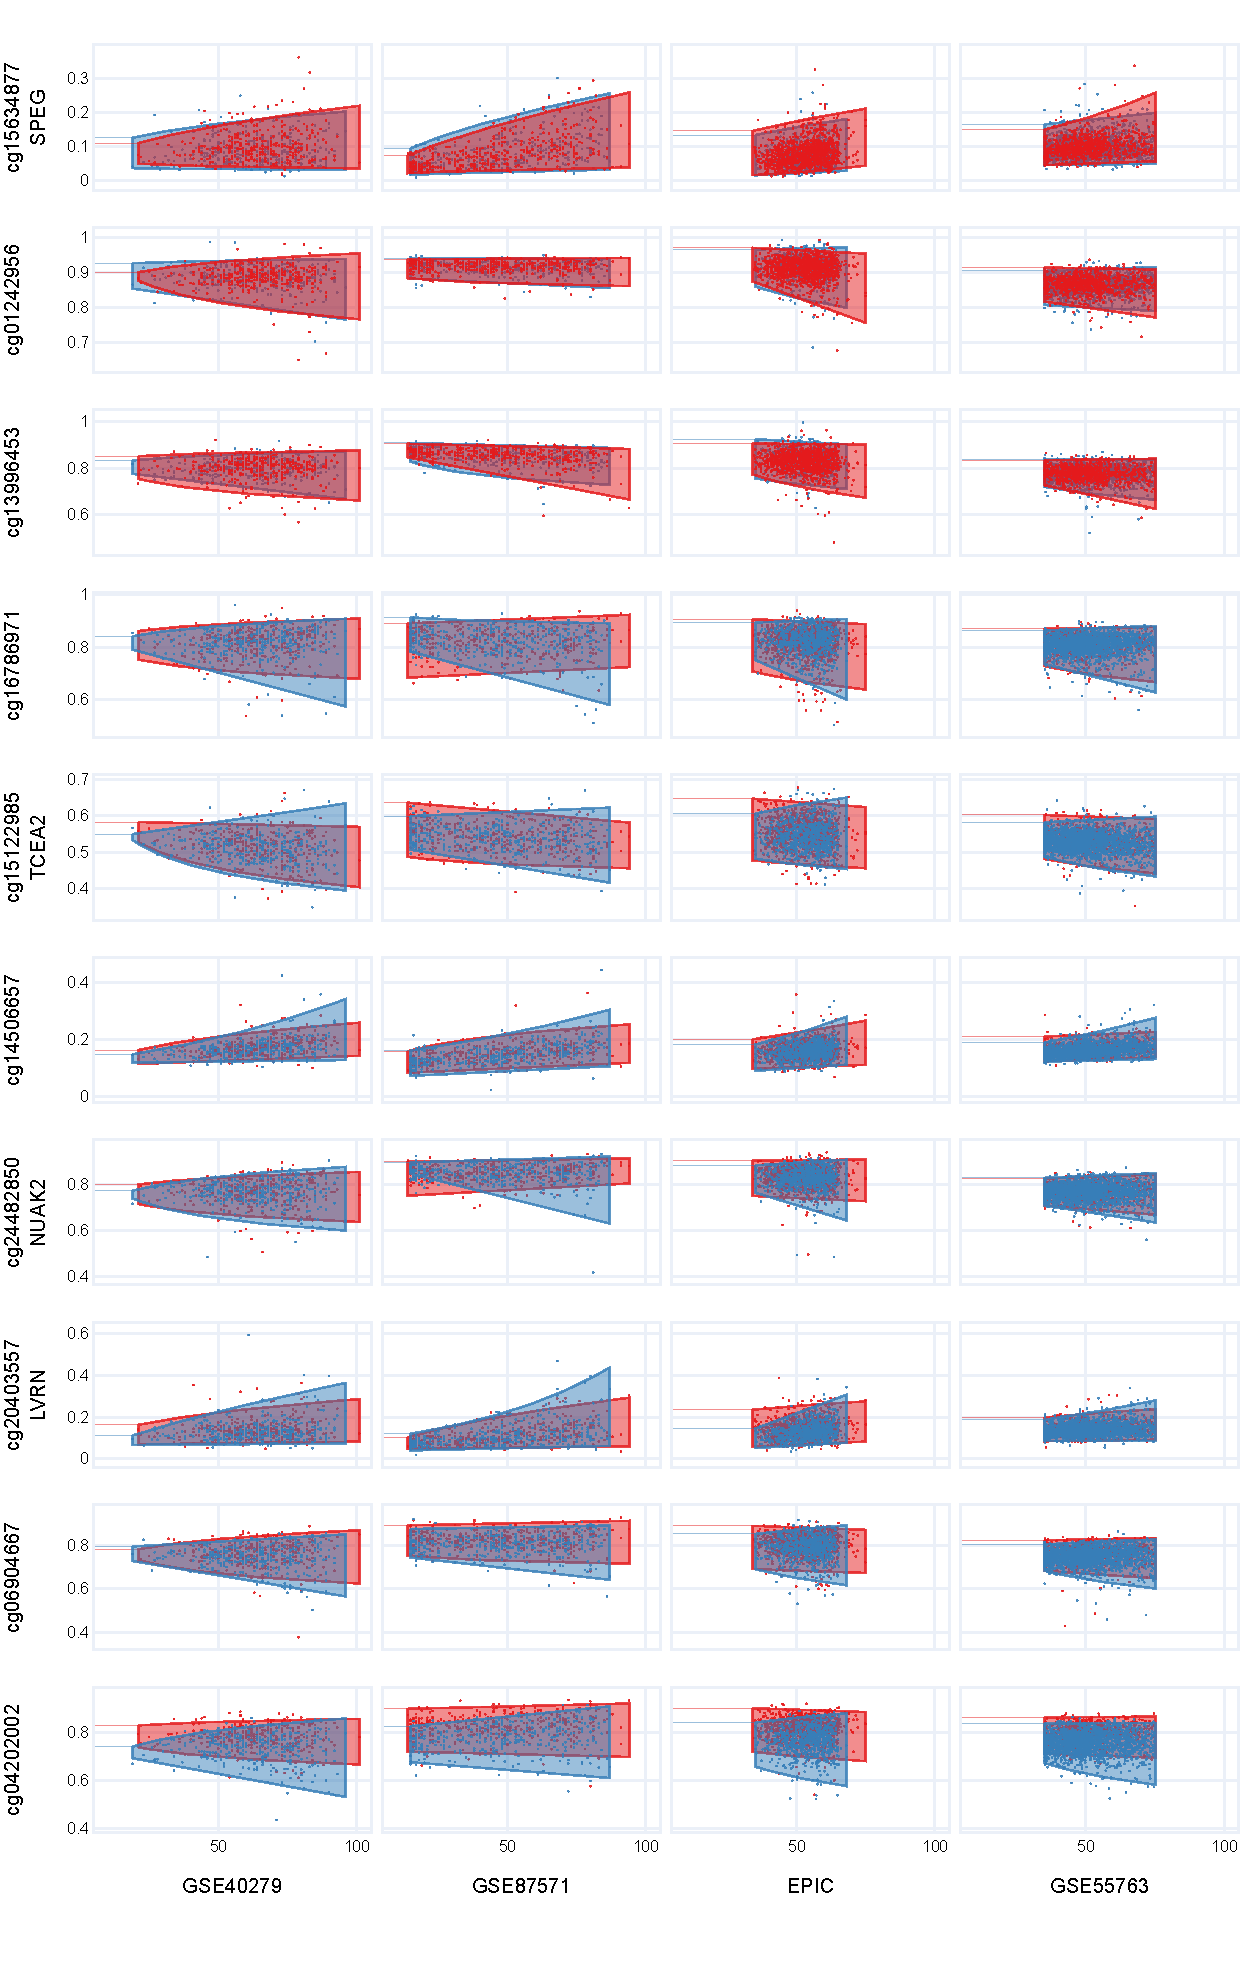
\includegraphics[scale=0.7]{saVMP.pdf}
	}
	\caption[Диаграммы разброса отдельных saVMP в четырёх рассматриваемых наборах данных.]{Диаграммы разброса отдельных saVMP в четырёх рассматриваемых наборах данных.}\label{fig:saVMP}
\end{figure}

Полученный результат согласуется с тем, что наблюдается для экспрессии генов в гиппокампе самцов и самок мышей в разном возрасте \autocite{Mangold2017} в предположении, что потеря эпигенетического и транскрипционного контроля, которая происходит во время старения, более заметна у самцов, чем у самок. Соответственно, более конкретный поиск saVMP показал, что у мужчин количество проб, показывающих возрастные изменения вариабельности метилирования, выше, чем у женщин, и что подавляющее большинство этих проб демонстрируют увеличение возрастной вариабельности.

\section*{Выводы по главе 2} \label{sec:ch2/conclusion}                       
\addcontentsline{toc}{section}{Выводы по главе 2}    

В данной главе был описан предлагаемый автором метод поиска связанных с возрастом специфичных для пола биомаркеров с использованием метаанализа, включающий также раздельный поиск связанных с возрастом и специфичных для пола биомаркеров. Кроме того, в главе был предложен алгоритм поиска биомаркеров с возрастной вариабельностью, связанной с полом, с использованием тестирования на гетероскедастичность. Разработанные методы реализованы в виде программного пакета для языка Python и доступен в репозитории Python Package Index (https://pypi.org/project/pydnameth). Для обоих методов проведена экспериментальная проверка работоспособности на реальных данных метилирования цельной крови, показана корректность получаемых результатов \autocite{Yusipov2020}.

\FloatBarrier
